\HIDE{
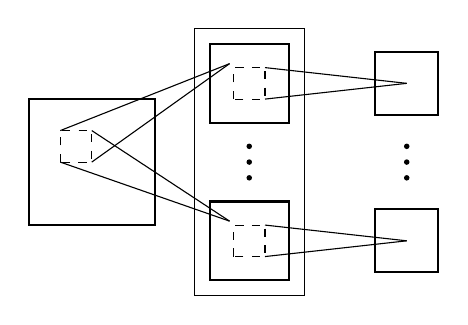
\begin{tikzpicture}
    \draw[thick] (-8mm,-8mm) rectangle (8mm,8mm);
    \draw[dashed] (-4mm, 0mm) rectangle (0mm,4mm);

    \draw[thick] (15mm,  5mm) rectangle ++(10mm,10mm);
    \foreach\y in {-2,0,2}
    {   \fill (20mm,1mm*\y) circle (1pt);
    }
    \draw[thick] (15mm,-15mm) rectangle ++(10mm,10mm);

    \draw (13mm,-17mm) rectangle (27mm,17mm);

    \draw (-4mm,4mm) -- (20mm-2.5mm, 10mm+2.5mm);
    \draw (20mm-2.5mm, 10mm+2.5mm) -- (0mm,0mm);
    \draw (0mm,4mm) -- (20mm-2.5mm,-10mm+2.5mm);
    \draw (20mm-2.5mm,-10mm+2.5mm) -- (-4mm,0mm);

    \draw[thick] (36mm, 6mm) rectangle ++(8mm,8mm);
    \foreach\y in {-2,0,2}
    {   \fill (40mm,1mm*\y) circle (1pt);
    }
    \draw[thick] (36mm,-14mm) rectangle (44mm,-6mm);

    \foreach\y in {-10,10}
    {   \draw[dashed] (18mm,1mm*\y-2mm) rectangle ++(4mm,4mm);
        \draw (22mm,1mm*\y+2mm) -- (40mm,1mm*\y);
        \draw (40mm,1mm*\y) -- (22mm,1mm*\y-2mm);
    }
\end{tikzpicture}
}
\begin{tikzpicture}
    [   kerline/.style =
        {   line join=round
        ,   densely dotted
        },
        kernel/.style =
        {   draw
        ,   circle
        ,   densely dotted
        }
    ]
    \newcommand{\kerlines}[2]{%
        \draw[kerline] (tangent cs:node=#1,point={(#2)},solution=1)
            -- (#2) -- (tangent cs:node=#1,point={(#2)},solution=2);
    }
    \newcommand{\kerdots}[1]{%
        \foreach\y in {-2,0,2}
        {   \fill (#1,1mm*\y) circle (1pt);
        }
    }

    %% planes
    % U0
    \node (U0) at ( 0mm,  0mm) [draw,rectangle,minimum size=20mm] {};
    % US1
    \node (US1G1) at (28mm,-15mm) [draw,rectangle,minimum size=16mm] {};
    \kerdots{28mm}
    \node (US1G2) at (28mm, 15mm) [draw,rectangle,minimum size=16mm] {};
    \draw (18mm,-25mm) rectangle (38mm,25mm);
    \node at (28mm,25mm) [above] {$U_{S1}$};
    % UC1
    \node (UC1G1) at (53mm,-15mm) [draw,rectangle,minimum size=14mm] {};
    \kerdots{53mm}
    \node (UC1G2)at (53mm, 15mm) [draw,rectangle,minimum size=14mm] {};
    \draw (44mm,-24mm) rectangle (62mm,24mm);
    \node at (53mm,24mm) [above] {$U_{C1}$};
    % US2
    \node (US2G1) at (75mm,-15mm) [draw,rectangle,minimum size=10mm] {};
    \kerdots{75mm}
    \node (US2G2) at (75mm, 15mm) [draw,rectangle,minimum size=10mm] {};
    \draw (68mm,-22mm) rectangle (82mm,22mm);
    \node at (75mm,22mm) [above] {$U_{S2}$};
    % UC2
    \node (UC2G1) at (94mm,-15mm) [draw,rectangle,minimum size=8mm] {};
    \kerdots{94mm}
    \node (UC2G2) at (94mm, 15mm) [draw,rectangle,minimum size=8mm] {};
    \draw (88mm,-21mm) rectangle (100mm,21mm);
    \node at (94mm,21mm) [above] {$U_{C2}$};

    %% kernels
    % U0 -> US1
    \coordinate (U0tUS1) at (-4mm,+4mm);
    \node[kernel] (U0K) at ($(U0)+(U0tUS1)$)
        [inner sep=0pt,minimum size=3mm] {};
    \coordinate (US1P1) at ($(US1G1)+(U0tUS1)$);
    \coordinate (US1P2) at ($(US1G2)+(U0tUS1)$);
    \kerlines{U0K}{US1P1}
    \kerlines{U0K}{US1P2}
    % US1 -> UC1
    \coordinate (US1tUC1) at (-4mm,-4mm);
    \node[kernel] (US1K1) at ($(US1G1)+(US1tUC1)$)
        [inner sep=0pt,minimum size=2mm] {};
    \node[kernel] (US1K2) at ($(US1G2)+(US1tUC1)$)
        [inner sep=0pt,minimum size=2mm] {};
    \coordinate (UC1P1) at ($(UC1G1)+(US1tUC1)$);
    \coordinate (UC1P2) at ($(UC1G2)+(US1tUC1)$);
    \kerlines{US1K1}{UC1P1}
    \kerlines{US1K2}{UC1P2}
    % UC1 -> US2
    \coordinate (UC1tUS2) at (-2mm,2mm);
    \node[kernel] (UC1K1) at ($(UC1G1)+(UC1tUS2)$)
        [inner sep=0pt,minimum size=3mm] {};
    \node[kernel] (UC1K2) at ($(UC1G2)+(UC1tUS2)$)
        [inner sep=0pt,minimum size=3mm] {};
    \coordinate (US2P1) at ($(US2G1)+(UC1tUS2)$);
    \coordinate (US2P2) at ($(US2G2)+(UC1tUS2)$);
    \kerlines{UC1K1}{US2P1}
    \kerlines{UC1K1}{US2P2}
    \kerlines{UC1K2}{US2P1}
    \kerlines{UC1K2}{US2P2}
    % US2 -> UC2
    \coordinate (US2tUC2) at (2mm,2mm);
    \node[kernel] (US2K1) at ($(US2G1)+(US2tUC2)$)
        [inner sep=0pt,minimum size=2mm] {};
    \node[kernel] (US2K2) at ($(US2G2)+(US2tUC2)$)
        [inner sep=0pt,minimum size=2mm] {};
    \coordinate (UC2P1) at ($(UC2G1)+(US2tUC2)$);
    \coordinate (UC2P2) at ($(UC2G2)+(US2tUC2)$);
    \kerlines{US2K1}{UC2P1}
    \kerlines{US2K2}{UC2P2}

    \foreach\x in {106,108,110}
    {   \fill (1mm*\x,0mm) circle (1pt);
    }
\end{tikzpicture}
